\documentclass[11pt, a4paper]{article}

\usepackage[brazil]{babel}
\usepackage[utf8]{inputenc}
\usepackage[T1]{fontenc}
\usepackage[pdftex]{hyperref}
\usepackage{graphicx}
\usepackage{amsmath}
\usepackage{indentfirst}
\usepackage{fancyhdr}


% Formatação
\topmargin -1.5cm
\oddsidemargin -0.04cm
\evensidemargin -0.04cm
\textwidth 16.59cm
\textheight 21.94cm 
%\pagestyle{empty}                     % Sem numero de paginas
\pagestyle{fancy}                         %cabecalhos e rodares
\fancyhead[RO,RE]{\today}
\fancyhead[LO,LE]{MAC0332 - SI para grupos de pesquisa\\
	Design}
\fancyfoot[LO,LE]{Confidential}
\fancyfoot[RO,RE] {\thepage}
\fancyfoot[CO,CE]{Grupo 3, 2011}


\parskip 7.2pt                        % Espaço entre paragrafos 7.2
%\renewcommand{\baselinestretch}{1.5} % Espaçamento entre linhas = 1.5
%\parindent 0pt

% Tirar hifenização
\hyphenpenalty = 5000
\tolerance = 1000
\sloppy

\title{MAC 0332\\
	Engenharia de Software\\
	SI para grupos de pesquisa\\
	Design}
\date{\today}

\begin{document}

	\maketitle
	\newpage
	
	\section{Estrutura do Design}
		%[Describe the design from the highest level. This is commonly done with a diagram that shows a layered architecture.]
		
		\begin{figure}[h]
            \center
            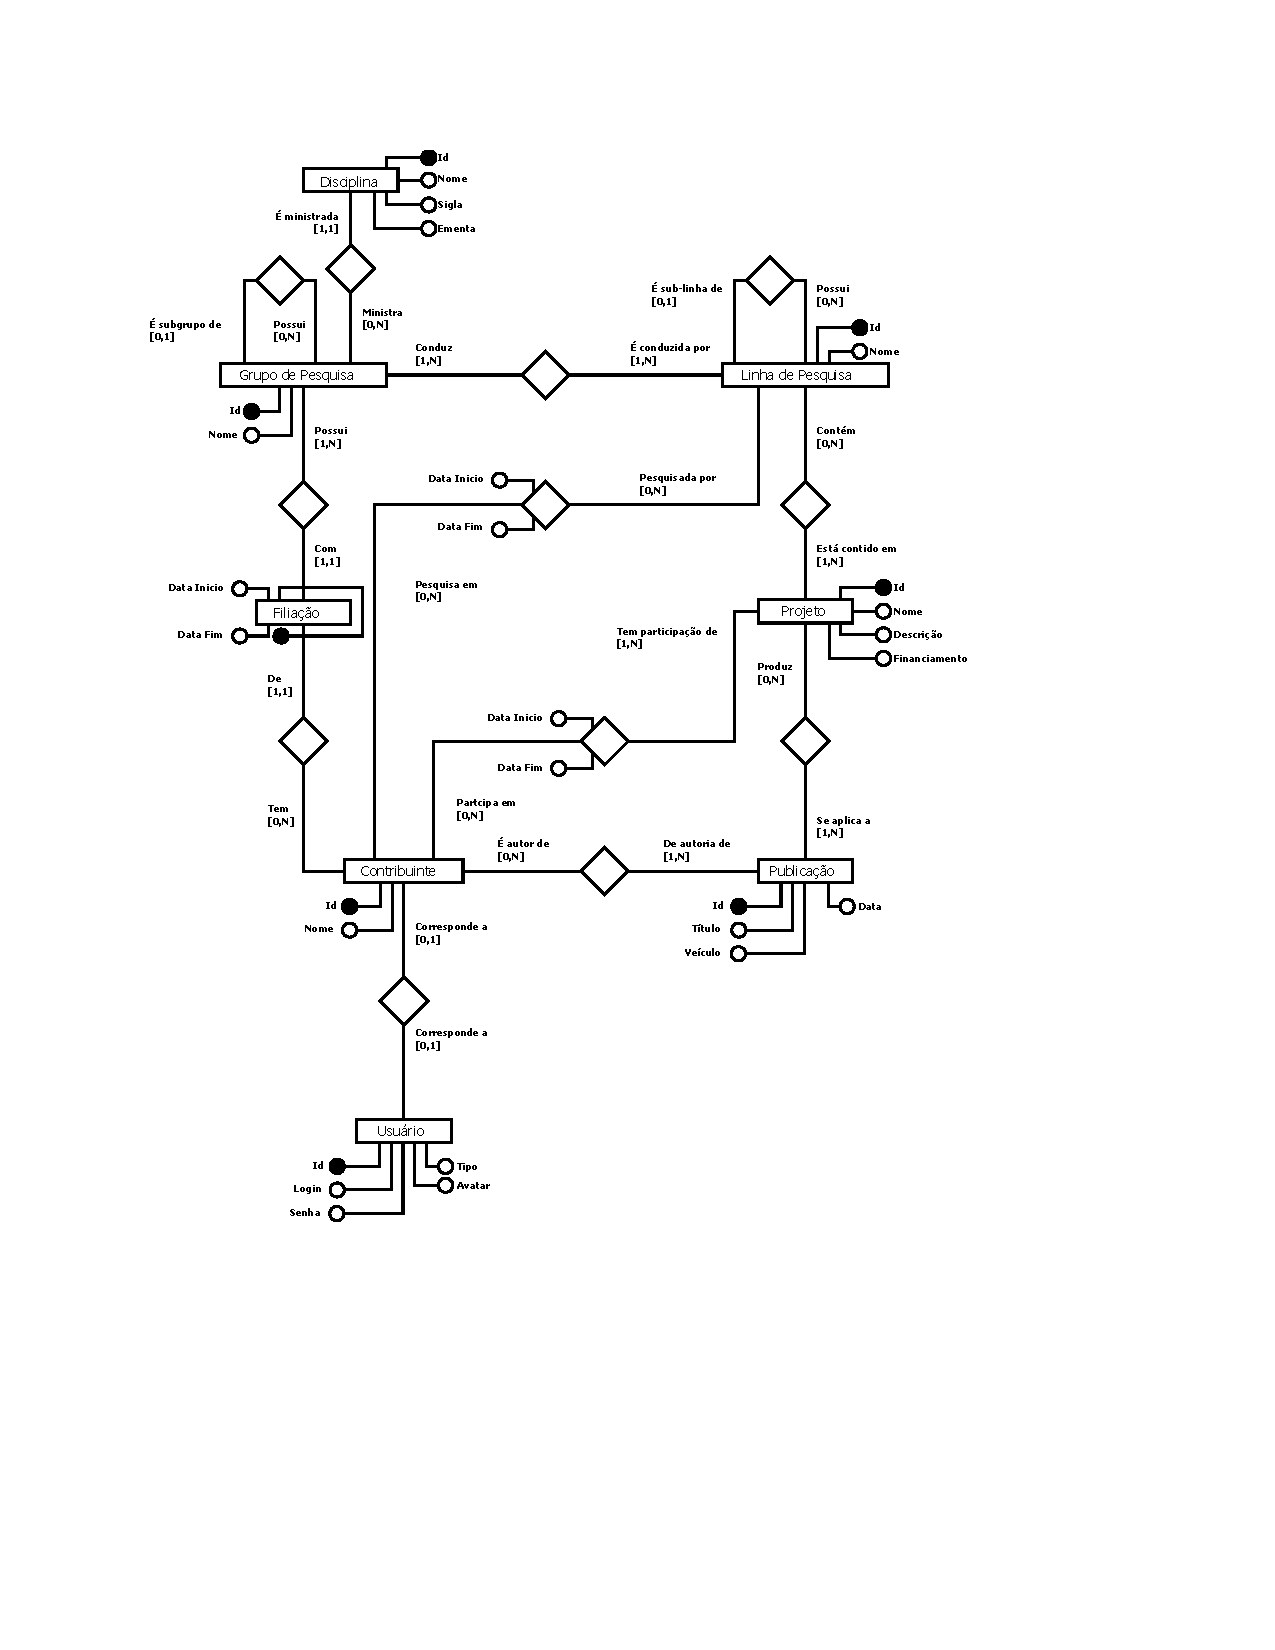
\includegraphics[width=12cm]{SIGP-DER.pdf}
            \label{DER}
            \caption{DER do Sistema}
        \end{figure}
        \newpage
        
		\begin{figure}[h]
            \center
            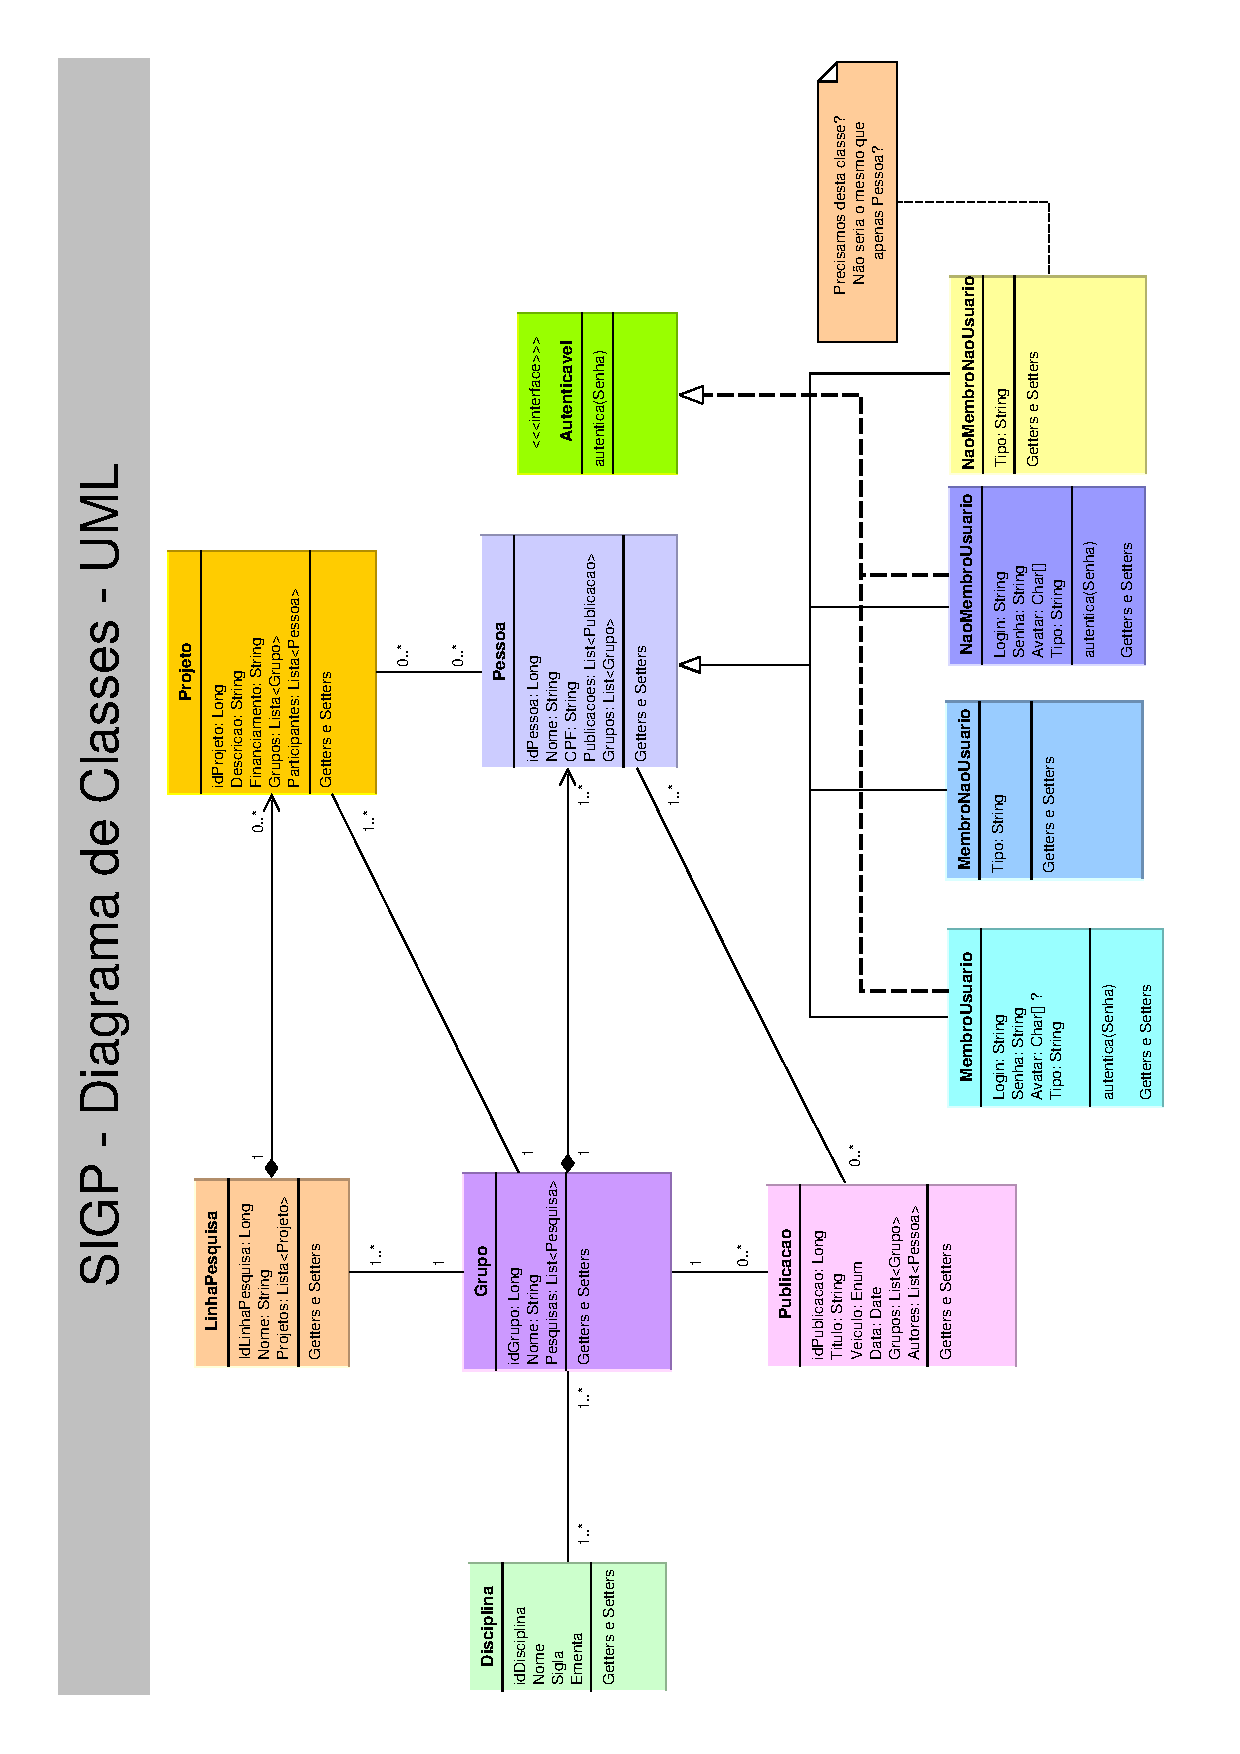
\includegraphics[width=12cm, angle=270]{SIGP-UML-classes.pdf}
            \label{DiagramaDeClasses}
            \caption{Diagrama de Classes}
        \end{figure}
		\newpage
		
	\section{Subsistemas}
	
        %[Describe the design of a portion of the system (a package or component, for instance). The design should capture both static and dynamic perspectives. When capturing dynamic descriptions of behavior, look for reusable chunks of behavior that you can reference to simplify the design of the requirement realizations. You can break this section down into lower-level subsections to describe lower-level, encapsulated subsystems.]
            \subsection{Subsistema  de Login}
                Precocupa-se em descobrir se um usuario é cadastrado, se é administrador, etc. Para isso busca no banco de dados, com senhas criptografadas, se o nome de usuario e senha digitadas coincidem, dano também a opção de se cadastrar u novo usuario.
            
            \subsection{Subsistema dos CRUD's}
                CRUD é uma abreviação de "Create, read, update and delete", temos esses para todass as classes do modelo, ou seja, podemos criar, listar, atualizar e remover qualquer objeto por meio de uma interface com o usuario.
            
	\section{Padrões}
        \subsection{Padrão 1}
		
		    \subsubsection{Visão Global}
                %[Provide an overview of the pattern in words in some consistent form. The overview of a pattern can include the intent, motivation, and applicability.]
		
		    \subsubsection{Estrutura}
                %[Describe the pattern from a static perspective. Include all of the participants and how they relate to one another, and call out the relevant data and behavior.]
		
		    \subsubsection{Comportamento}
                %[Describe the pattern from a dynamic perspective. Walk the reader through how the participants collaborate to support various scenarios.]
		
		    \subsubsection{Exemplo}
		        %[Often, you can convey the nature of the pattern better with an additional concrete example.]
		        
		\subsection{Padrão 2}
		
		    \subsubsection{Visão Global}
                %[Provide an overview of the pattern in words in some consistent form. The overview of a pattern can include the intent, motivation, and applicability.]
		
		    \subsubsection{Estrutura}
                %[Describe the pattern from a static perspective. Include all of the participants and how they relate to one another, and call out the relevant data and behavior.]
		
		    \subsubsection{Comportamento}
                %[Describe the pattern from a dynamic perspective. Walk the reader through how the participants collaborate to support various scenarios.]
		
		    \subsubsection{Exemplo}
		        %[Often, you can convey the nature of the pattern better with an additional concrete example.]
		        
		\subsection{Padrão.....}		
		    ......

		
	\section{Realizações de Exigência}
        
        \subsection{Listagem dos CRUD's}
		
	        \subsubsection{Visão dos Participantes}
                %[Describe the participating design elements from a static perspective, giving details such as behavior, relationships, and attributes relevant to this realization.]
                Todas as listagens foram implementadas usando Hiberante e VRaptor, na loinguagem Java.
		
	        \subsubsection{Cenário Básico}
                %[For the main flow, describe how instances of the design elements collaborate to realize the requirements. When using UML, this can be done with collaboration diagrams (sequence or communication).]
                O Hibernate criar os bancos de dados, depois de criado, fazemos uma pesquisa do dado CRUD e usamos o VRaptor para fazer a visualização final da pagina.
					
             
        \subsection{Cadastro de novo grupo e suas relações}
		
	        \subsubsection{Visão dos Participantes}
                %[Describe the participating design elements from a static perspective, giving details such as behavior, relationships, and attributes relevant to this realization.]
                Administrador cadastra um grupo, que pode ser subgrupo de um grupo maior, um membro do grupo cadastra uma publicação e pode dizer a quais projetos aquela publicação se aplica. Isso tudo foi feito usando o conjunto Hibernate VRaptor, para pesquisa e gravação no Banco de Dados.

	        \subsubsection{Cenário Básico}
                %[For the main flow, describe how instances of the design elements collaborate to realize the requirements. When using UML, this can be done with collaboration diagrams (sequence or communication).]
                A patir do VRaptor chamamos o Hibernate e com sua retorno da pesquisa mostramos os resultados no pagina final.

\end{document}
